\documentclass[12pt]{article}

\setlength{\parskip}{1em}

\usepackage[T1]{fontenc}
\usepackage[french]{babel}
\usepackage{enumitem}
\usepackage{textcomp}
\usepackage{amsfonts}
\usepackage{slantsc}
\usepackage{graphicx}
\usepackage{amsmath}
\usepackage[a4paper, margin=1in]{geometry}

\usepackage{hyperref}
\hypersetup{
  colorlinks=true,
  linkcolor=blue,
  urlcolor=blue,
  pdftitle={Projet LO21: Rapport final}
}

\usepackage{listings}
\lstset{
  numbers=left,
  columns=fullflexible,
  language=C,
  numberstyle=\scriptsize,
}

\usepackage[linesnumbered, french]{algorithm2e}
\SetKwInput{Data}{Donn\'ees}
\SetKwInput{Result}{R\'esultat}
\SetKwInput{Vars}{Variables}
\SetKwInput{Assertion}{Assertion}
\SetKwInput{KWClass}{Classe}
\newcommand{\Class}[1]{\KWClass{$\mathcal{O}(#1)$}}
\SetKwIF{If}{ElseIf}{Else}{Si}{alors}{Sinon si}{Sinon}{FinSi}
\SetKwFor{While}{Tant que}{faire}{Fin TantQue}
\SetKwBlock{Begin}{D\'ebut}{Fin}
\SetKwBlock{BeginKB}{D\'ebut BC}{Fin BC}
\SetKwRepeat{Repeat}{Faire}{Tant que}
\DontPrintSemicolon
\SetAlgoLined

\RestyleAlgo{boxruled}

\newcommand{\Assign}[2]{#1 $\; \longleftarrow \;$ #2}
\newcommand{\Arg}[2]{\hspace{0.2em}#1\hspace{0.05em}: #2}
% \newcommand{\Child}[2]{(#1 $\rightarrow$ #2)}
\newcommand{\Child}[2]{#2(#1)}
\newcommand{\Null}[0]{\textsc{null}\hspace{4pt}}
\newcommand{\Et}[2]{#1\hspace{2pt}\textnormal{\textbf{et}}\hspace{2.5pt}#2}
\newcommand{\Not}[1]{\textnormal{\textbf{non}}(#1)}
% \newcommand{\Neither}[2]{\Et{\Not{#1}}{\Not{#2}}}

\renewcommand{\arraystretch}{1.5}

\title{Projet LO21: Rapport final \\ \large \og Système Expert \fg}
\author{Adrien Burgun}
\date{Automne 2020}
\graphicspath{{report/}}

\begin{document}

\maketitle

\begin{abstract}

  Le projet de ce semestre pour le cours de \textbf{LO21} (Algorithmique et Programmation II) porte sur un \textit{\og système expert \fg}.
  Un système expert est constitué de 3 éléments:

  \begin{description}[align=left]
    \item [Une base de connaissance,] qui prend la forme suivante:
    \[
      A \land B \land ... \land Z \Rightarrow \Omega
    \]
    Où \(A, B, ...\) sont les symboles (d'arité zéro, aussi appelés \og propositions \fg) constituant la \textit{prémisse} et \(\Omega\) est la \textit{conclusion}.

    \item [Une base de faits,] qui est la liste des symboles ayant la valeur \textit{\og Vrai \fg} (qui correspond à l'état \textit{\og Certain \fg}). \\
    Un symbole ne faisant pas partie de cette liste a par défaut la valeur \textit{\og Faux \fg} (qui correspond à l'état \textit{\og Incertain \fg}).

    \item [Un moteur d'inférence,] qui, à partir de la base de connaissance et la base de faits, déduit quels autres symboles sont aussi vrais et les ajoute à la base de faits.
  \end{description}

  Nous définirons d'abords le type \textit{\og Règle \fg}, constituant les éléments de la base de connaissance, puis le type \textit{\og BC \fg} (\underline{B}ase de \underline{C}onnaissance), ainsi que les fonctions leur étant associés. \\
  Nous décrirons ensuite le moteur d'inférence comme implémenté dans ce projet, avec différents exemples de l'éxecution de celui-ci. \\
  Nous verrons enfin comment nous avons pu étendre ce moteur d'inférence à l'algèbre booléen.

\end{abstract}

\newpage
\tableofcontents
\newpage

% 1
\section{Règles}

Soit \textbf{Règle} le type représentant une règle sous la forme d'une liste de symboles:

% Faire un tableau?

% \begin{lstlisting}
% #define LONGUEUR_SYMBOLE 256

% struct regle {
%   char symbole[LONGUEUR_SYMBOLE];
%   struct regle* suivant;
% };

% typedef struct regle regle_t;
% \end{lstlisting}

\begin{tabular}{|p{3cm}|p{4cm}|p{6.5cm}|}
  \hline
  \multicolumn{3}{|c|}{\textbf{Structure 1 :} Règle\label{R}} \\
  \hline
  \textbf{Nom} & \textbf{Type} & \textbf{Description} \\
  \hline
  \textit{symbole} & Règle $\rightarrow$ Symbole & Retourne le nom du symbole correspondant au noeud en tête de liste. \\
  \hline
  \textit{suivant} & Règle $\rightarrow$ Règle & Retourne une référence au prochain élément de la liste, \textit{règle\_vide} si l'élément est le dernier de la liste. \\
  \hline
  \textit{nouvelle\_règle} & ((Symbole) $\times$ Règle) $\rightarrow$ Règle & Compose une nouvelle règle à partir du nom d'un symbole et une référence à la prochaine règle. \\
  \hline
  \textit{règle\_vide} & Règle & La règle vide. \\
  \hline
  \textit{mettre\_suivant} & (Règle $\times$ Règle) $\rightarrow$ Règle & Modifie une Règle pour y attacher une Règle comme règle suivante; retourne également la règle modifiée. \\
  \hline
\end{tabular}

Le type \og Symbole \fg correspond dans l'implémentation C à une chaîne de caractères.
Le dernier élément d'une telle liste correspond à la conclusion de la règle, tandis que tous les autres éléments appartiennent à la prémisse (contrainte du projet).

Les axiomes sur ces fonctions sont:

\begin{itemize}
\item \textit{symbole}(\textit{nouvelle\_règle}(s, r)) = s
\item \textit{suivant}(\textit{nouvelle\_règle}(s, r)) = r
\item \Assign{A}{\textit{nouvelle\_règle}(s, r)}; \textit{mettre\_suivant}(a, r') $\; \Rightarrow$ \textit{suivant}(A) = r'
\end{itemize}

Nous pouvons noter que:

Liste $\prec$ Règle [$\emptyset$: \textit{règle\_vide}, tête: \textit{symbole}, reste: \textit{suivant}, insérer\_tête: \textit{nouvelle\_règle}, Élement: Symbole]

(Soit également un type concret implémentant Règle implémente également Liste(Symbole))

Nous avons implémenté ce type abstrait de donnée sous forme d'une liste chaînée, de part sa facilité d'implémentation et la difficulté d'implémenter un type abstrait de donnée grandissable par la tête sous tout autre forme qu'une liste chaînée.

Le fait que ce type abstrait soit grandissable par la tête reflète également la difficulté de décrire de manière concise et simple à comprendre toute autre forme de type abstrait représentant une liste.

% 1.1
\subsection{Créer une règle vide}

Nous représentons une règle vide par \textit{règle\_vide}.
Voici l'algorithme permettant de créer une règle vide:

\begin{algorithm}[H]
\Vars{\Arg{$R$}{La règle vide à retourner}}
\Result{\Arg{$R$}{Règle}}
\Class{1}

\Begin({RègleVide()}){
  \Assign{$R$}{\textit{règle\_vide}}
}

\caption{RègleVide\label{RV}}
\end{algorithm}

% 1.2
\subsection{Ajouter une proposition à la prémisse d'une règle}

% Je me permets d'interrompre votre brave lecture de ce document latex pour argumenter sur la question posée dans le sujet original, qui stipule que cet ajout doit se faire en *queue*, et non pas en *tête*.
% Voici donc des exemples d'utilisations de cette fonction et les résultats auxquels on s'attendrait (1) par rapport aux résultats qu'on obtiendra avec cette contrainte (2):
%
% ajout_prémisse(ø, A) -> (1) A | ø, (2) ø | A
% ajout_prémisse(ø | A, B) -> (1) B | A; (2) A | B
% ajout_prémisse(A & B | Ω, C) -> (1) C & A & B | Ω; (2) A & B & Ω | C
%
% Le problème est, à mon avis, qu'ajouter un symbole à la prémisse d'une règle ne devrait pas affecter la conclusion d'une règle, ce qui n'est pas le cas lorsque l'ajout se fait à l'endroit dédié à la conclusion de la règle.
% Cela voudra aussi dire que la fonction pour ajouter une conclusion à une règle sera identique à celle-ci.
%
% PS: après plusieures semaines de travail sur ce projet, je pense que le sujet attendait que l'on utilise une liste grandissable en queue pour Règle, et que l'on décrive ses fonctions de manière sémantique, et non de manière axiomatique.

L'ajout des propositions (symboles) à la prémisse d'une règle se fait par l'algorithme \textit{AjoutPrémisse} défini ci-dessous.
Cet ajout se fait en queue de la liste (contrainte du projet).

La liste donnée en entrée est modifiée par l'algorithme et est ensuite retournée; ceci est dû aux contraintes des listes chaînées dans l'implémentation C et du type abstrait de donnée Règle: si la liste est initialement vide (représenté par \Null et \textit{règle\_vide}), alors nous ne pouvons pas muter celle-ci en utilisant \textit{mettre\_suivant}.
Ceci est géré par le premier \textbf{Si}.

\newpage

\begin{algorithm}[H]
\Vars{
  \begin{itemize}
    \item \Arg{$R$}{La règle à modifier}
    \item \Arg{$R'$}{Une variable temporaire pour traverser la liste}
    \item \Arg{\textit{symbole}}{Le nom de la proposition (symbole) à insérer}
  \end{itemize}
}
\Data{\Arg{$R$}{Règle}, \Arg{\textit{symbole}}{Symbole}}
\Result{\Arg{$R$}{Règle}}
\Assertion{$R$ n'a pas encore de conclusion}
\Class{n}

\Begin({AjoutPrémisse($R$, \textit{symbole})}){
  \uIf{$R$ = \textit{règle\_vide}}{
    \Assign{$R$}{\textit{nouvelle\_règle}(\textit{symbole}, \textit{règle\_vide})}
  }
  \Else{
    \Assign{$R'$}{R}

    \tcp{Répeter jusqu'à ce qu'on atteigne le dernier élément}

    \While{\Child{$R'$}{\textit{suivant}} $\neq$ \textit{règle\_vide}}{
      \Assign{$R'$}{\Child{$R'$}{\textit{suivant}}}
    }

    \tcp{$R'$ contient désormais le dernier élément de la liste}

    \textit{mettre\_suivant}($R'$, \textit{nouvelle\_règle(\textit{symbole}, \textit{règle\_vide})})
  }
}

\caption{AjoutPrémisse\label{AP}}
\end{algorithm}

% 1.3
\subsection{Créer la conclusion d'une règle}

Créer la conclusion d'une règle revient à ajouter une proposition (symbole) à la fin de la règle.
Pour ce faire, nous ré-utilisons l'algorithme \hyperref[AP]{AjoutPrémisse} défini plus tôt.

\begin{algorithm}[H]
\Vars{
  \begin{itemize}
    \item \Arg{$R$}{La règle à modifier}
    \item \Arg{\textit{symbole}}{Le nom de la proposition (symbole) à insérer comme conclusion}
  \end{itemize}
}
\Data{\Arg{$R$}{Règle}, \Arg{\textit{symbole}}{Symbole}}
\Result{\Arg{$R$}{Règle}}
\Assertion{$R$ n'a pas encore de conclusion}
\Class{n}

\Begin({AjoutConclusion($R$, \textit{symbole})}){
  \Assign{$R$}{\hyperref[AP]{AjoutPrémisse}($R$, \textit{symbole})}
}

\caption{AjoutConclusion\label{AC}}
\end{algorithm}

% 1.4
\subsection{Tester si une proposition appartient à la prémisse d'une règle}

Nous testons si une proposition appartient à la prémisse d'une règle en traversant celle-ci de manière récursive (contrainte du projet).

Les 3 cas minimaux sont:

\begin{description}
  \item[$R$ = {[]}] (règle vide): retourner \og Faux \fg
  \item[$R$ = \{symbole: "...", suivant: \textit{règle\_vide}\}] (conclusion): retourner \og Faux \fg
  \item[$R$ = \{symbole: symbole\_recherché, suivant: ...\}] (symbole trouvé): retourner \og Vrai \fg
\end{description}

Dans les autres cas, nous retournons de manière récursive le résultat de la même fonction, appelée sur \Child{$R$}{\textit{suivant}}.

\begin{algorithm}[H]
\Vars{
  \begin{itemize}
    \item \Arg{$R$}{La règle à étudier}
    \item \Arg{\textit{symbole}}{La nom de la proposition à rechercher}
    \item \Arg{\textit{résultat}}{Si oui ou non la proposition à été trouvée}
  \end{itemize}
}
\Data{\Arg{$R$}{Règle}, \Arg{\textit{symbole}}{Symbole}}
\Result{\Arg{\textit{résultat}}{Booléen}}
\Assertion{$R$ a une conclusion}
\Class{n}

\Begin({TestAppartenance($R$, \textit{symbole})}){
  \uIf{$R$ = \textit{règle\_vide}}{
    \tcp{Règle vide}
    \Assign{\textit{résultat}}{Faux}
  }
  \uElseIf{\Child{$R$}{\textit{suivant}} = \textit{règle\_vide}}{
    \tcp{Conclusion}
    \Assign{\textit{résultat}}{Faux}
  }
  \uElseIf{\Child{$R$}{\textit{symbole}} = \textit{symbole}}{
    \tcp{Symbole trouvé}
    \Assign{\textit{résultat}}{Vrai}
  }
  \Else{
    \Assign{\textit{résultat}}{TestAppartenance(\Child{$R$}{\textit{suivant}}, \textit{symbole})}
  }
}

\caption{TestAppartenance\label{TA}}
\end{algorithm}

% 1.5
\subsection{Supprimer une proposition de la prémisse d'une règle}

Nous supprimons une proposition de la prémisse d'une règle de manière récursive.
Cette décision est motivée par le format de Règle et sa simplicité d'implémentation.
Les cas minimaux sont les suivants:

\begin{description}
  \item[$R$ = {[]}] (règle vide): retourner \textit{règle\_vide}
  \item[$R$ = \{symbole: "...", suivant: \textit{règle\_vide}\}] (conclusion): retourner $R$
\end{description}

Dans le cas général, nous attribuons à \Child{$R$}{\textit{suivant}} la valeur retournée par cette fonction, appelée sur \Child{$R$}{\textit{suivant}}, puis nous retournons soit \Child{$R$}{\textit{suivant}} si le noeud correspond au symbole, soit $R$ sinon.

\begin{algorithm}[H]
\Vars{
  \begin{itemize}
    \item \Arg{$R$}{La règle à modifier}
    \item \Arg{\textit{symbole}}{La nom de la proposition à rechercher}
    \item \Arg{$R'$}{La règle privée de \textit{symbole} dans sa prémisse}
  \end{itemize}
}
\Data{\Arg{$R$}{Règle}, \Arg{\textit{symbole}}{Symbole}}
\Result{\Arg{$R'$}{Règle}}
\Assertion{$R$ a une conclusion}
\Class{n}

\Begin({SupprimerSymbole($R$, \textit{symbole})}){
  \uIf{$R$ = \textit{règle\_vide}}{
    \tcp{Règle vide}
    \Assign{$R'$}{\textit{règle\_vide}}
  }
  \uElseIf{\Child{$R$}{\textit{suivant}} = \textit{règle\_vide}}{
    \tcp{Conclusion}
    \Assign{$R'$}{$R$}
  }
  \Else{
    \uIf{\Child{$R$}{\textit{symbole}} = \textit{symbole}}{
      \tcp{Retourner le reste de la liste, sans ce noeud}
      \Assign{$R'$}{SupprimerSymbole(\Child{$R$}{\textit{suivant}}, \textit{symbole})}
    }
    \Else{
      \Assign{$R'$}{\textit{mettre\_suivant}($R$, SupprimerSymbole(\Child{$R$}{\textit{suivant}}, \textit{symbole}))}
    }
  }
}

\caption{SupprimerSymbole\label{SS}}
\end{algorithm}

% 1.6
\subsection{Tester si la prémisse d'une règle est vide}

Voici la fonction retournant \og Vrai \fg si la prémisse d'une règle est vide et \og Faux \fg si la prémisse d'une règle contient au moins 1 symbole:

\begin{algorithm}[H]
\Vars{
  \begin{itemize}
    \item \Arg{$R$}{La règle à étudier}
    \item \Arg{\textit{résultat}}{Si oui ou non la prémisse d'une règle est vide}
  \end{itemize}
}
\Data{\Arg{$R$}{Règle}}
\Result{\Arg{\textit{résultat}}{Booléen}}
\Assertion{$R$ a une conclusion ou $R$ est vide}
\Class{1}

\Begin({PrémisseVide($R$)}){
  \uIf{$R$ = \textit{règle\_vide}}{
    \tcp{La règle est vide, donc sa prémisse est vide}
    \Assign{\textit{résultat}}{Vrai}
  }
  \uElseIf{\Child{$R$}{\textit{suivant}} = \textit{règle\_vide}}{
    \tcp{La règle n'a qu'une conclusion, donc sa prémisse est vide}
    \Assign{\textit{résultat}}{Vrai}
  }
  \Else{
    \Assign{\textit{résultat}}{Faux}
  }
}

\caption{PrémisseVide\label{PV}}
\end{algorithm}

% 1.7
\subsection{Accéder à la proposition se trouvant en tête d'une prémisse}

Voici la fonction retournant la valeur de la proposition se trouvant en tête d'une prémisse.
Si la prémisse est vide, alors la fonction retourne \textit{symbole\_vide} ($\emptyset$).

\begin{algorithm}[H]
\Vars{
  \begin{itemize}
    \item \Arg{$R$}{La règle à étudier}
    \item \Arg{\textit{résultat}}{La valeur du premier symbole de la prémisse, si existant}
  \end{itemize}
}
\Data{\Arg{$R$}{Règle}}
\Result{\Arg{\textit{résultat}}{Symbole}}
\Assertion{$R$ a une conclusion}
\Class{1}

\Begin({TêteRègle($R$)}){
  \uIf{\hyperref[PV]{PrémisseVide}($R$)}{
    \tcp{La prémisse est vide: nous retournons \textit{symbole\_vide}}
    \Assign{\textit{résultat}}{\textit{symbole\_vide}}
  }
  \Else{
    \Assign{\textit{résultat}}{\Child{$R$}{\textit{symbole}}}
  }
}

\caption{TêteRègle\label{TR}}
\end{algorithm}

% 1.8
\subsection{Accéder à la conclusion d'une règle}

La conclusion se trouvant à la fin d'une règle, nous traversons simplement la liste jusqu'au dernier élément de celle-ci et retournons sa valeur.
Si la liste est vide, alors la fonction retourne \textit{règle\_vide}.

\begin{algorithm}[H]
\Vars{
  \begin{itemize}
    \item \Arg{$R$}{La règle à étudier}
    \item \Arg{$R'$}{Variable temporaire pour traverses la liste}
    \item \Arg{\textit{résultat}}{La valeur du premier symbole de la prémisse, si existant}
  \end{itemize}
}
\Data{\Arg{$R$}{Règle}}
\Result{\Arg{\textit{résultat}}{Symbole}}
\Assertion{$R$ a une conclusion}
\Class{n}

\Begin({ConclusionRègle($R$)}){
  \uIf{\Child{$R$}{\textit{suivant}} = \textit{règle\_vide}}{
    \Assign{\textit{résultat}}{\textit{règle\_vide}}
  }
  \Else{
    \Assign{$R'$}{$R$}

    \tcp{Avançer jusqu'à la fin de la liste}
    \While{\Child{$R'$}{\textit{suivant}} $\neq$ \textit{règle\_vide}}{
      \Assign{$R'$}{\Child{$R'$}{\textit{suivant}}}
    }

    \Assign{\textit{résultat}}{\Child{$R'$}{\textit{symbole}}}
  }
}

\caption{ConclusionRègle\label{CR}}
\end{algorithm}

% 2
\section{Base de Connaissance}

Soit \textbf{BC} le type représentant une base de connaissance (liste de règle); celle-ci prend la forme d'une liste de Règles:

\begin{tabular}{|p{3cm}|p{4cm}|p{6.5cm}|}
  \hline
  \multicolumn{3}{|c|}{\textbf{Structure 2 :} BC\label{BC}} \\
  \hline
  \textbf{Nom} & \textbf{Type} & \textbf{Description} \\
  \hline
  \textit{règle} & BC $\rightarrow$ Règle & Retourne une référence à la règle correspondant à ce noeud. \\
  \hline
  \textit{suivant} & BC $\rightarrow$ BC & Une référence au prochain élément de la liste, \Null si l'élément est le dernier de la liste. \\
  \hline
  \textit{nouvelle\_base} & (Règle $\times$ BC) $\rightarrow$ BC & Crée une nouvelle base à partir d'une référence vers une Règle et d'une référence vers BC \\
  \hline
  \textit{base\_vide} & BC & La base vide \\
  \hline
\end{tabular}

Les axiomes sur ces fonctions sont:

\begin{itemize}
  \item \textit{règle}(\textit{nouvelle\_base}(r, b)) = r
  \item \textit{suivant}(\textit{nouvelle\_base}(r, b)) = b
\end{itemize}

Pour les même raisons que celles de Règle, le type abstrait BC est grandissable par la tête et son implémentation proposée se fait sous la forme d'une liste chaînée.

% 2.1
\subsection{Créer une base vide}

Nous représentons une base vide par \textit{base\_vide}.
Voici l'algorithme permettant de créer une base vide:

\begin{algorithm}[H]
\Vars{\Arg{$B$}{La base vide à retourner}}
\Result{\Arg{$B$}{BC}}
\Class{1}

\Begin({BaseVide()}){
  \Assign{$B$}{\textit{base\_vide}}
}

\caption{BaseVide\label{BV}}
\end{algorithm}

% 2.2
\subsection{Ajouter une règle à une base de connaissance}

L'ajout de règle à la base de connaissance se fait en tête (pour sa simplicité d'implémentation). Voici son algorithme:

\begin{algorithm}[H]
\Vars{
  \begin{itemize}
    \item \Arg{$B$}{La base de connaissance à modifier}
    \item \Arg{\textit{règle}}{La valeur de \textit{règle} à mettre dans le noeud}
    \item \Arg{$B'$}{La base de connaissance contenant la nouvelle règle}
  \end{itemize}
}
\Data{\Arg{$B$}{BC}; \Arg{\textit{règle}}{Règle}}
\Result{\Arg{$B'$}{BC}}
\Class{1}

\Begin({AjoutRègle($B$, \textit{règle})}){
  \Assign{$B'$}{\textit{nouvelle\_base}(\textit{règle}, $B$)}
}

\caption{AjoutRègle\label{AR}}
\end{algorithm}

% 2.3
\subsection{Accéder à la règle se trouvant en tête de la base}

Voici l'algorithme permettant d'accéder à la règle se trouvant en tête; s'il n'y a pas de règle en tête, nous retournons \textit{règle\_vide}.

\begin{algorithm}[H]
\Vars{
  \begin{itemize}
    \item \Arg{$B$}{La base de connaissance à modifier}
    \item \Arg{$R$}{La règle se trouvant en tête de la base, \textit{règle\_vide} si la base est vide}
  \end{itemize}
}
\Data{\Arg{$B$}{BC}}
\Result{\Arg{$R$}{Règle}}
\Class{1}

\Begin({TêteBase($B$)}){
  \uIf{$B$ = \textit{base\_vide}}{
    \Assign{$R$}{\textit{règle\_vide}}
  }
  \Else{
    \Assign{$R$}{\textit{règle}($B$)}
  }
}

\caption{TêteBase\label{TB}}
\end{algorithm}

\newpage

\section{Moteur d'inférence}

Le moteur d'inférence est un algorithme permettant de déduire à partir de la liste initiale des symboles (propositions) ayant la valeur \og Vrai \fg et de la base de connaissance (BC) la liste de tous les symboles étant vrais.

L'algorithme éxecute un maximum de $n$ (la longueur de la base de connaissance) passages sur les règles, celles-cis prenant la forme suivante ($p \geq 0$ symboles $S_x$ dans la prémisse et le symbole $\Omega_k$ dans la conclusion; le symbole $\land$ correspond à \og et \fg):

\[BC \vdash (\bigwedge_{x=0}^{x < p} S_x) \Rightarrow \Omega_k\]

\[\text{Avec: } \quad (\bigwedge_{x=0}^{x < p} S_x) = \begin{cases}
  S_0 \land S_1 \land ... \land S_{p-1} & \text{Si } p > 0 \\
  Vrai & \text{Si } p = 0
\end{cases}
\]

Si $\Omega_k$ n'appartient pas encore à la liste des symboles vrais et que $\forall x \in [0, p[, S_x = Vrai$ ou $p = 0$, alors on ajoute $\Omega_k$ à la liste des symboles vrais.

Nous notons par la suite $n$ pour la longueur de la base de connaissance, $p$ pour la longueur maximale des règles de la base de connaissance et $q$ pour le nombre de symboles différents faisant partie de la base de connaissance ou étant initiallement présents dans $S$.
Nous assumons que les symboles ont une longueur maximale fixée au préalable, faisant de leur comparaison une fonction de classe $\mathcal{O}(1)$.

\begin{algorithm}
\Vars{
  \begin{itemize}
    \item \Arg{$B$}{La base de connaissance, de longueur $n$ et dont les règles ont pour longueur maximale $p$.}
    \item \Arg{$B'$}{Variable temporaire pour traverser la base de connaissance}
    \item \Arg{$S$}{La liste des symboles initialements vrais}
    \item \Arg{$S'$}{La liste des symboles initialement vrais ainsi que ceux déduits des règles d'induction}
    \item \Arg{\textit{ajouté}}{Si oui ou non un symbole à été rajouté à $S'$ dans le dernier passage}
  \end{itemize}
}
\Data{\Arg{$B$}{BC}; \Arg{$S$}{Liste(Symbole)}}
\Result{\Arg{$S'$}{Liste(Symbole)}}
\Assertion{$\forall R \in B, R \neq$ \textit{règle\_vide}}
\Class{n^2 \cdot q \cdot p}

\Begin({MoteurInférence($B$, $S$)}){
  \Assign{$S'$}{$S$}

  \tcp{\underline{Boucle principale}: Répétée jusqu'à ce qu'il n'y aie plus de modification à $S'$ possibles}
  \Repeat{\textit{ajouté}}{
    \Assign{\textit{ajouté}}{Faux} \\
    \Assign{$B'$}{$B$}

    \tcp{Pour toutes les règles de la base de connaissance...}
    \While{$B' \neq$ \textit{base\_vide}}{
      \tcp{Si la conclusion n'appartient pas à $S'$...}
      \If{\Not{\hyperref[LC]{ListeContient}($S'$, \hyperref[CR]{ConclusionRègle}(\hyperref[TB]{TêteBase}($B'$)))}}{
        \tcp{Si la prémisse est vraie, alors on ajoute la conclusion à $S'$}
        \If{\hyperref[PVr]{PrémisseVraie}(\hyperref[TB]{TêteBase}($B'$), $S'$)}{
          \Assign{$S'$}{\textit{insérer\_tête}($S'$, \hyperref[CR]{ConclusionRègle}(\hyperref[TB]{TêteBase}($B'$)))} \\
          \Assign{\textit{ajouté}}{Vrai}
        }
      }
      \Assign{$B'$}{\textit{suivant}($B'$)}
    }
  }
}

\caption{MoteurInférence\label{MI}}
\end{algorithm}

\begin{algorithm}
\Vars{
  \begin{itemize}
    \item \Arg{$T$}{Un type d'objets comparables}
    \item \Arg{$L$}{Une liste d'objets de type $T$}
    \item \Arg{$E$}{La valeur à trouver dans $L$}
    \item \Arg{\textit{résultat}}{Si oui ou non $E$ est trouvé dans $L$}
  \end{itemize}
}
\Data{\Arg{$L$}{Liste($T$)}; \Arg{$E$}{$T$}}
\Result{\Arg{\textit{résultat}}{Booléen}}
\Class{longueur(L)}

\Begin({ListeContient($L$, $E$)}){
  \uIf{\textit{est\_vide}($L$)}{
    \Assign{\textit{résultat}}{Faux}
  }
  \uElseIf{\textit{tête}($L$) = $E$}{
    \Assign{\textit{résultat}}{Vrai}
  }
  \Else{
    \Assign{\textit{résultat}}{ListeContient(\textit{reste}($L$), $E$)}
  }
}

\caption{ListeContient\label{LC}}
\end{algorithm}


\begin{algorithm}
\Vars{
  \begin{itemize}
  \item \Arg{$S$}{La liste de symboles vrais, de longueur maximale $q$}
  \item \Arg{$R$}{La règle à vérifier, de longueur maximale $p$}
  \item \Arg{$R'$}{Variable utilisée pour traverser $R$}
  \item \Arg{\textit{résultat}}{Si oui ou non la prémisse de la règle est vraie}
  \end{itemize}
}
\Data{\Arg{$R$}{Règle}; \Arg{$S$}{Liste(Symbole)}}
\Result{\Arg{\textit{résultat}}{Booléen}}
\Assertion{$R \neq$ \textit{règle\_vide}}
\Class{p \cdot q}

\Begin({PrémisseVraie($R$, $S$)}){
  \Assign{\textit{résultat}}{Vrai}

  \If{\Not{\hyperref[PV]{PrémisseVide}($R$)}}{
    \Assign{$R'$}{$R$}

    \While{\Et{\textit{suivant}($R'$) $\neq$ \textit{règle\_vide}}{\textit{résultat}}}{
      \If{\Not{\hyperref[LC]{ListeContient}($S$, \hyperref[TR]{TêteRègle}($R'$))}}{
        \Assign{\textit{résultat}}{Faux}
      }

      \Assign{$R'$}{\textit{suivant}($R'$)}
    }
  }
}

\caption{PrémisseVraie\label{PVr}}
\end{algorithm}

\newpage

\section{Jeux d'essais}

\RestyleAlgo{plain}

Voici quelques jeux d'essais pour tester les capacités du moteur d'inférence.
Ceux-cis peuvent être retrouvés dans le fichier \textbf{src/test.c} (utilisant les fonctions décrites jusqu'ici).

Pour simplifier la lecture de ceux-cis, nous omettrons les algorithmes permettant de générer la base de connaissance et fournirons à la place une représentation visuelle de celle-ci.

\subsection{Test basique}

Ce premier essai est un essai très simple, visant à vérifier le bon fonctionnement des fonctions \hyperref[PV]{PrémisseVraie} et \hyperref[MI]{MoteurInférence}.
Le symbole $C$ ne doit être ajouté que si $A$ et $B$ sont vrais; dans les autres cas, la liste d'entrée reste intouchée.

\begin{algorithm}
\BeginKB(Test 1\label{T1}){
  $A \land B \Rightarrow C$
}
\end{algorithm}

\begin{tabular}{|p{4cm}|p{6.5cm}|}
  \hline
  \multicolumn{2}{|c|}{\textbf{Test 1 :}} \\
  \hline
  \textbf{Symboles d'entrée} & \textbf{Symboles de sortie} \\
  \hline
  $\emptyset$ & $\emptyset$ \\
  \hline
  $A$ & $A$ \\
  \hline
  $B$ & $B$ \\
  \hline
  $A, B$ & $A, B, \mathbf{C}$ \\
  \hline
\end{tabular}

\subsection{Somme égale à 2}

Ce test ajoute le symbole $D$ à la liste de sortie si 2 symboles parmis $A$, $B$ et $C$ sont présents ($A, B$ ou $A, C$ ou $B, C$).
Ce test vise à vérifier le bon fonctionnement du \hyperref[MI]{moteur d'inférence}: plusieures règles peuvent avoir la même conclusion, permettant de simuler l'opérateur $\lor$ (correspondant à \og ou \fg).

\begin{algorithm}
\BeginKB(Test 2\label{T2}){
  $A \land B \Rightarrow D$ \\
  $A \land C \Rightarrow D$ \\
  $B \land C \Rightarrow D$ \\
}
\end{algorithm}

Ces trois règles peuvent être réduites à $(A \land B) \lor (A \land C) \lor (B \land C) \Rightarrow D$.

\begin{tabular}{|p{4cm}|p{6.5cm}|}
  \hline
  \multicolumn{2}{|c|}{\textbf{Test 2:}} \\
  \hline
  \textbf{Symboles d'entrée} & \textbf{Symboles de sortie} \\
  \hline
  $A, B$ & $A, B, \mathbf{D}$ \\
  \hline
  $A, C$ & $A, C, \mathbf{D}$ \\
  \hline
  $B, C$ & $B, C, \mathbf{D}$ \\
  \hline
  $A, B, C$ & $A, B, C, \mathbf{D}$ \\
  \hline
\end{tabular}

\subsection{Distributivité du \og et \fg}

Ce test tente de prouver que $(A \lor B) \land C \Rightarrow (A \land C) \lor B$.
Pour ce faire, les deux moitiés de l'implication sont séparés en deux symboles \og cibles \fg, $D$ et $E$:

\begin{algorithm}
\BeginKB{
  $(A \lor B) \land C \Rightarrow D$ \\
  $(A \land C) \lor B \Rightarrow E$
}
\end{algorithm}

Nous devons ensuite réecrire ces deux règles sous le format accepté par le moteur d'inférence; nous faisons la substitution $tmp \equiv (A \lor B)$ et distribuons les $\lor$ sur les $\Rightarrow$:

\begin{algorithm}
\BeginKB(Test 3\label{T3}){
  \tcp{Partie gauche}
  $A \Rightarrow tmp$ \\
  $B \Rightarrow tmp$ \\
  $tmp \land C \Rightarrow D$ \\

  \tcp{Partie droite}
  $A \land C \Rightarrow E$ \\
  $B \Rightarrow E$
}
\end{algorithm}

Il nous suffit ensuite de vérifier que $D \rightarrow E$ pour les 8 différentes combinaisons de $A$, $B$ et $C$:

\begin{tabular}{|p{4cm}|p{6.5cm}|}
  \hline
  \multicolumn{2}{|c|}{\textbf{Test 3:}} \\
  \hline
  \textbf{Symboles d'entrée} & \textbf{Symboles de sortie} \\
  \hline
  $\emptyset$ & $\emptyset$ \\
  \hline
  $A$ & $A, \mathbf{tmp}$ \\
  \hline
  $B$ & $B, \mathbf{tmp}, \mathbf{E}$ \\
  \hline
  $A, B$ & $A, B, \mathbf{tmp}, \mathbf{E}$ \\
  \hline
  $C$ & $C$ \\
  \hline
  $A, C$ & $A, C, \mathbf{tmp}, \mathbf{D}, \mathbf{E}$ \\
  \hline
  $B, C$ & $B, C, \mathbf{tmp}, \mathbf{D}, \mathbf{E}$ \\
  \hline
  $A, B, C$ & $A, B, C, \mathbf{tmp}, \mathbf{D}, \mathbf{E}$ \\
  \hline
\end{tabular}

Nous pouvons observer dans les trois derniers cas que si $D$ est présent, alors $E$ est présent.
$D$ n'étant pas présents dans les 5 autres cas, notre théorème est vérifié.

\section{Extension du moteur d'inférence}

Comme nous l'avons vu précédemment, nous pouvons facilement introduire le symbole $\lor$ (\og ou \fg) et éxecuter différentes transformations pour arriver à un ensemble de règles ne contenant que les opérateurs $\land$ et $\Rightarrow$.

L'implémentation de ce projet contient une telle extension (que vous pourrez trouver dans le dossier \textbf{ext}), introduisant \href{https://github.com/adri326/lo21-project/blob/main/ext/grammar.ebnf}{un langage} dédié à celle-ci.
Cette extension introduit aussi l'opérateur $\neg$ (\og non \fg) et l'opérateur $\Leftrightarrow$ (\og ssi \fg).

Nous pouvons appliquer les opérations de simplification suivantes pour passer de ce langage utilisant les opérateurs \((\lor, \land, \neg, \Rightarrow, \Leftrightarrow)\) au langage utilisant uniquement les opérateurs \((\land, \neg, \Rightarrow)\), en se basant sur la logique classique:

\begin{itemize}
  \item $\neg(A \land B) \; \mapsto \; \neg{A} \lor \neg{B} \quad [A, B]$
  \item $\neg(A \lor B) \; \mapsto \; \neg{A} \land \neg{B} \quad [A, B]$
  \item $A \lor B \Rightarrow C \; \mapsto \; (A \Rightarrow C), (B \Rightarrow C) \quad [A, B, C]$
  \item $A \Rightarrow C \land D \; \mapsto \; (A \Rightarrow C), (A \Rightarrow D) \quad [A, C, D]$
  \item $\neg \neg A \; \mapsto \; A \quad [A]$
  \item $A \Leftrightarrow B \; \mapsto \; (A \Rightarrow B), (\neg A \Rightarrow \neg B) \quad [A, B]$
\end{itemize}

Une fois ces simplifications appliquées, nous obtenons un ensemble de règle que le \hyperref[MI]{moteur d'inférence} peut comprendre.

\subsection{Implémentation}

L'implémentation de l'extension lit et analyse un fichier écrit dans le langage dédié et le transforme par distributivité du $\land$ en un ensemble de règles du format:

\[BC^{*} \vdash (\bigvee_{x=0}^{x < p}\bigwedge_{y=0}^{y < p'_x} S_{x,y}) \Rightarrow \bigwedge_{x=0}^{y < q} T_x\]

Tel que:

\begin{align}
  \forall x (\bigwedge_{y=0}^{y < p'_x} S_{x,y})
    &= S_{x,0} \land S_{x,1} \land ... \land S_{x,p\-1} \\
  (\bigvee_{x=0}^{x < p} S_x')
    &= \begin{cases}
      S_0' \lor S_1' \lor ... \lor S_{p-1}' & \text{Si } p > 0 \\
      Vrai & \text{Si } p = 0
    \end{cases} \\
  \forall (x, y), S_{x,y}
    &= \begin{cases}
      S \in \textit{Symbole} & \text{Symbole non-inversé} \\
      \neg S \in \neg \textit{Symbole} & \text{Symbole inversé}
    \end{cases} \\
  \bigwedge_{x=0}^{y < q} T_x
    &= T_0 \land T_1 \land ... \land T_{q-1} \\
  \forall x, T_x
    &= \begin{cases}
      S \in \textit{Symbole} & \text{Symbole non-inversé} \\
      \neg S \in \neg \textit{Symbole} & \text{Symbole inversé}
    \end{cases} \\
  \forall x, p'_x &> 0 \\
  q &> 0
\end{align}

Les simplifications sont ensuite appliquées pour arriver à un ensemble de règles du \hyperref[MI]{format accepté par le moteur d'inférence}, avec pour différence que l'ensemble des symboles est étendu à $Symbole^{*} = Symbole \; \cup \; \neg Symbole$.
Lors de cette simplification, le programme est également capable de transformer la majorité des règles en leurs règles opposées.

Le programme attend enfin que l'utilisateur entre une ou plusieures commandes, celles-ci éxecutant le moteur d'inférence avec différents symboles d'entrée.

\subsection{Exemple: distributivité du \og et \fg}

Similairement au \hyperref[T3]{Test 3}, nous pouvons exprimer la relation $(A \lor B) \land C \Rightarrow (A \land C) \lor B$ de cette manière, en utilisant cette fois-ci les symboles que l'extension nous propose:

\begin{algorithm}[H]
\BeginKB(Test 4\label{T4}){
  $(A \lor B) \land C \Leftrightarrow D$ \\
  $(A \land C) \lor B \Leftrightarrow E$ \\
  $(D \land E) \lor \neg D \Leftrightarrow \textit{résultat}$
}
\end{algorithm}

Cette base de donnée est encodée dans le langage de l'extension et lui est donnée en entrée, ce fichier est fourni avec ce projet, à l'adresse \href{https://github.com/adri326/lo21-project/blob/main/ext/test/test-3.kb}{\textbf{ext/test/test-3.kb}}.
Nous éxécutons ensuite le moteur d'inférence avec pour entrée les permutations de $A/\neg A$, $B/\neg B$ et $C/\neg C$:

\begin{tabular}{|p{4cm}|p{6.5cm}|}
  \hline
  \multicolumn{2}{|c|}{\textbf{Test 3:}} \\
  \hline
  \textbf{Symboles d'entrée} & \textbf{Symboles de sortie} \\
  \hline
  $\neg A, \neg B, \neg C$ & $\neg A, \neg B, \neg C, \mathbf{\neg D}, \mathbf{\neg E}, \textbf{résultat}$ \\
  \hline
  $A, \neg B, \neg C$ & $A, \neg B, \neg C, \mathbf{\neg D}, \mathbf{\neg E}, \textbf{résultat}$ \\
  \hline
  $\neg A, B, \neg C$ & $\neg A, B, \neg C, \mathbf{\neg D}, \mathbf{E}, \textbf{résultat}$ \\
  \hline
  $A, B, \neg C$ & $A, B, \neg C, \mathbf{\neg D}, \mathbf{E}, \textbf{résultat}$ \\
  \hline
  $\neg A, \neg B, C$ & $\neg A, \neg B, C, \mathbf{\neg D}, \mathbf{\neg E}, \textbf{résultat}$ \\
  \hline
  $A, \neg B, C$ & $A, \neg B, C, \mathbf{D}, \mathbf{E}, \textbf{résultat}$ \\
  \hline
  $\neg A, B, C$ & $\neg A, B, C, \mathbf{D}, \mathbf{E}, \textbf{résultat}$ \\
  \hline
  $A, B, C$ & $A, B, C, \mathbf{D}, \mathbf{E}, \textbf{résultat}$ \\
  \hline
\end{tabular}

\newpage

Voici le même résultat, géneré par le programme:

\begin{center}
  \makebox[\textwidth]{
    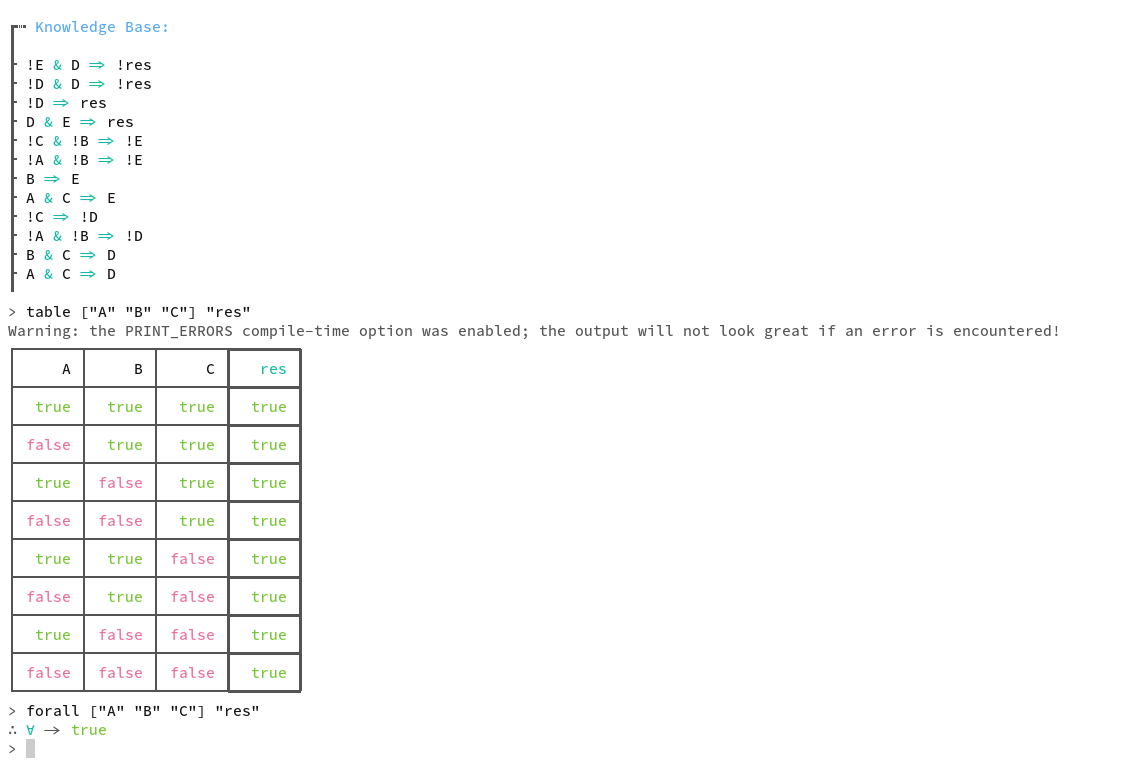
\includegraphics[width=\textwidth]{report/test-3-screenshot}
  }
\end{center}

\textbf{résultat} étant vrai dans tous les cas, le théorème $(A \lor B) \land C \Rightarrow (A \land C) \lor B$ est validé.

\newpage

\section{Conclusion}

Nous avons, pour ce projet, décrit le fonctionnement d'un système expert simple sous forme d'algorithme et implémenté celui-ci en langage C.
Nous avons aussi pu étendre ce système expert à l'ensemble de l'algèbre booléen et le munir d'un langage dédié et d'une interface interactive.

L'implémentation de base ainsi que son extension sont capables de prouver des théorèmes simples dans l'algèbre booléen, comme celui présenté en exemple.
Le moteur d'inférence a le désavantage d'être à minima de classe $\mathcal{O}(n^2)$ par rapport au nombre de règle, car il est obligé de les traverser une par une; nous pouvons imaginer que sur une grande base de connaissance, celui-ci risque de prendre longtemps.
Une optimisation possible serait d'indéxer les symboles au préalables et de ne s'y réferrer et les comparer que par leur indexe, ainsi que de supprimer les règles déjà atteintes lors du parcours de la base de connaissance.

Même si celui-ci peut être étendu, ce modèle de système expert reste limité, car il ne supporte que des symboles de type booléen.

\newpage
\RestyleAlgo{boxruled}
\listofalgorithms

\end{document}
